\documentclass{article}
\usepackage{amsmath}
\usepackage{graphicx}
\begin{document}
\author{Ana Bhattacharjee}
\title{Parallel and Perpendicular Lines: Question 15}
\date{\today}

\begin{center}
The triangle JKL is shown below.
\begin{figure}[!htbp]
  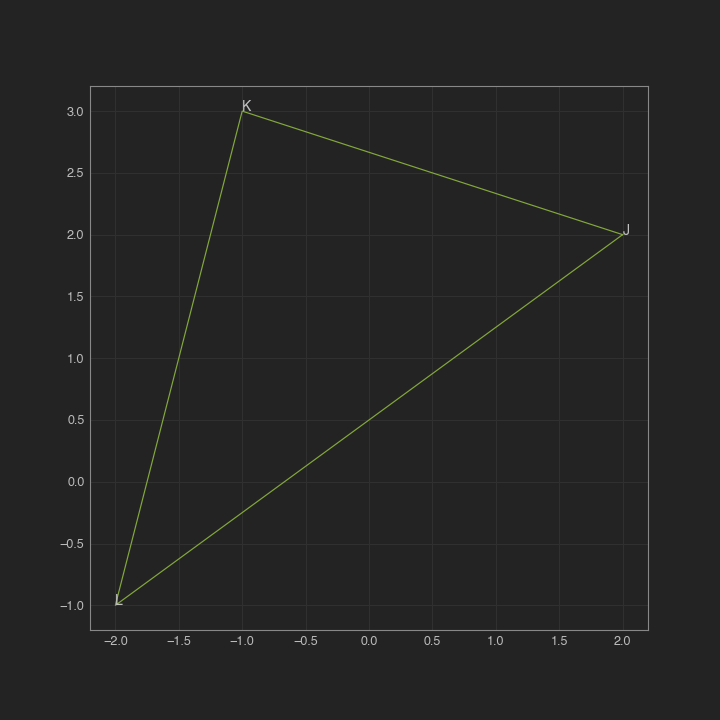
\includegraphics[width=1\columnwidth]{../q15}
  \caption{Triangle JKL}
\end{figure}
\par
To determine whether or not this triangle is a right triangle, I will calculate the slopes of JK and KL and see whether or not they are perpendicular to each other.
\par
\begin{align}
  \text{slope}_{JK} = \frac{3-2}{-1 - 2} = -\frac{1}{3} \\
  \text{slope}_{KL} = \frac{-1 - 3}{-2 - (-1)} = \frac{-4}{-1} = 4 \\
\end{align}
\par
Since the slopes are not negative reciprocols of eachother, the triangle JKL is not a right triangle. 
\end{center}
\end{document}
